\documentclass[11pt]{standalone}
\usepackage{amssymb}
\usepackage{amsmath}
\usepackage[no-math]{fontspec}
\usepackage{unicode-math}
\usepackage{libertinus}
\usepackage{pgf,xcolor}
\usepackage{tikz}
\usetikzlibrary{arrows.meta, backgrounds}
\usepackage{pgfplots}
\pgfplotsset{compat=newest}

\definecolor{my_darkgray}{HTML}{484949}
\definecolor{my_lightgray}{HTML}{F3F4F4}
\definecolor{my_darkblue}{HTML}{005A94}
\definecolor{my_lightblue}{HTML}{CCDEE9}
\definecolor{my_yellow}{HTML}{FFEC7F}
\definecolor{my_red}{HTML}{E60000}
\definecolor{my_orange}{HTML}{E87846}

\begin{document}
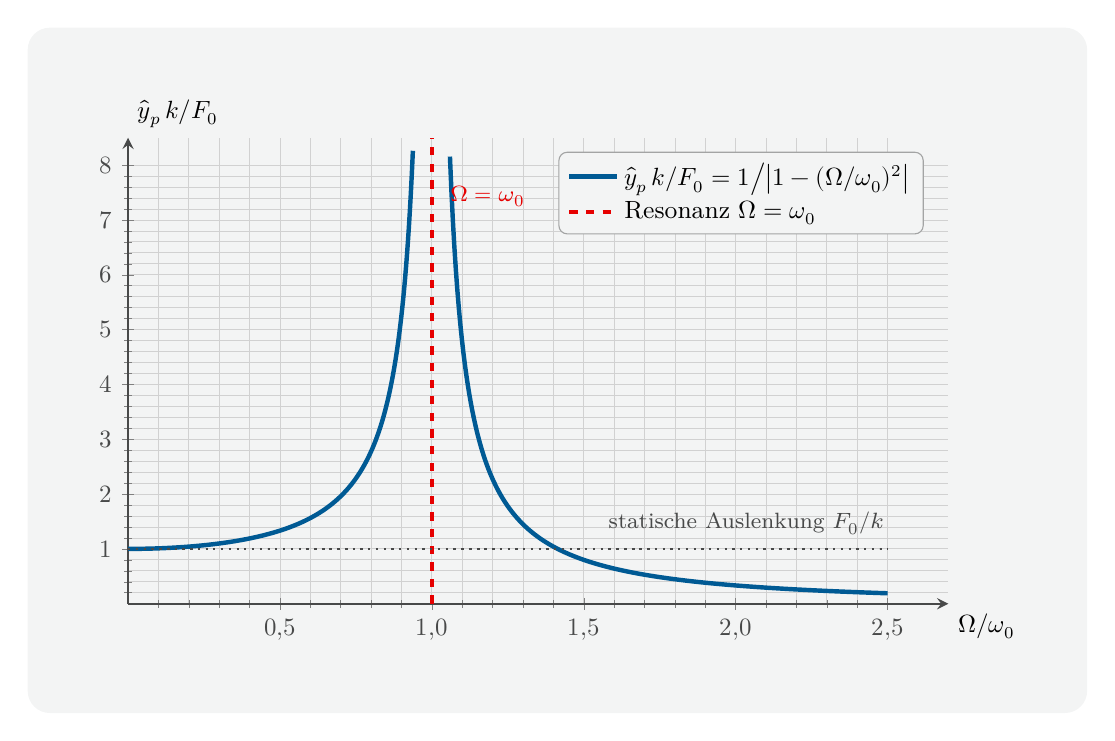
\begin{tikzpicture}[
    show background rectangle,
    background rectangle/.style={fill=my_lightgray, rounded corners=8pt},
    inner frame sep=0.8cm
]
\begin{axis}[
    % axis equal weggelassen: Ω/ω₀ ist dimensionslos und reicht von 0 bis 2,5;
    % ŷ_p·k/F₀ reicht von 0 bis 8 — gleiche Skalierung würde die Kurvenverläufe
    % stark verzerren und die Resonanzkurve unleserlich machen.
    axis lines=center,
    xlabel={$\Omega/\omega_0$},
    ylabel={$\hat{y}_p\,k/F_0$},
    xlabel style={at={(ticklabel* cs:1.0)}, anchor=north west, font=\small},
    ylabel style={at={(ticklabel* cs:1.0)}, anchor=south west, font=\small},
    grid=both,
    grid style={line width=0.3pt, draw=my_darkgray!25},
    axis line style={thick, draw=my_darkgray},
    width=12cm,
    height=7.5cm,
    xmin=0, xmax=2.7,
    ymin=0, ymax=8.5,
    xtick={0, 0.5, 1.0, 1.5, 2.0, 2.5},
    xticklabels={$0$, $0{,}5$, $1{,}0$, $1{,}5$, $2{,}0$, $2{,}5$},
    ytick={0, 1, 2, 3, 4, 5, 6, 7, 8},
    tick label style={font=\small, color=my_darkgray},
    minor tick num=4,
    samples=300,
    legend pos=north east,
    legend style={
        font=\small,
        fill=my_lightgray,
        draw=my_darkgray!50,
        rounded corners=3pt
    },
    legend cell align=left,
    clip=true,
]

%% --- Unterkritischer Ast: 0 ≤ Ω/ω₀ < 1 ---
%% V(r) = 1 / (1 − r²),  r = Ω/ω₀
%% restrict y to domain schützt vor Überläufen nahe der Polstelle.
\addplot[draw=my_darkblue, ultra thick, domain=0:0.96,
         restrict y to domain=0:8.5]
    {1 / (1 - x^2)};
\addlegendentry{$\hat{y}_p\,k/F_0 = 1\big/\bigl|1-(\Omega/\omega_0)^2\bigr|$}

%% --- Überkritischer Ast: Ω/ω₀ > 1 ---
%% Separater \addplot-Aufruf wegen der Polstelle bei r = 1 (kein eigener
%% Legendeneintrag, da es denselben Kurvenausdruck fortsetzt).
\addplot[draw=my_darkblue, ultra thick, domain=1.04:2.5,
         restrict y to domain=0:8.5, forget plot]
    {1 / (x^2 - 1)};

%% --- Vertikale Asymptote bei Ω = ω₀  (r = 1) ---
\addplot[draw=my_red, ultra thick, dashed]
    coordinates {(1, 0) (1, 8.5)};
\addlegendentry{Resonanz $\Omega = \omega_0$}

%% --- Waagerechte Referenzlinie: statische Auslenkung F₀/k  (r → 0) ---
\addplot[draw=my_darkgray, thick, dotted, domain=0:2.5, forget plot]
    {1};
\node[font=\footnotesize, text=my_darkgray, anchor=south west]
    at (axis cs: 1.55, 1.08)
    {statische Auslenkung $F_0/k$};

%% --- Annotation: kritische Drehzahl ---
\node[font=\footnotesize, text=my_red, anchor=north west]
    at (axis cs: 1.03, 7.8)
    {$\Omega = \omega_0$};

\end{axis}
\end{tikzpicture}
\end{document}
